\chapter[Resultados]{Resultados}

A partir do estudo e pesquisa realizado até o momento determinamos o que utilizar no conjunto do sistema, levantando um perfil que a equipe acredita ser a mais viável em termos de interação, custo-benefício, tempo, conhecimento técnico e outros fatores importantes para o projeto. Será desenvolvido um kit com capacidade de ser acoplado em diversas cadeiras de rodas afim de facilitar a mobilidade elétrica em cadeiras manuais. Os resultados levantados estão disposto no decorrer do capítulo.

\section{Estrutura}

Com a utilização do programa CATIA V5 3D foi estruturado o sistema eletrônico acoplado à cadeira de rodas, \ref{fig:vista_isometrica_traseira}. Visando três preceitos básicos: comodidade, acessibilidade e conforto.

\begin{figure}[!htb]
\centering
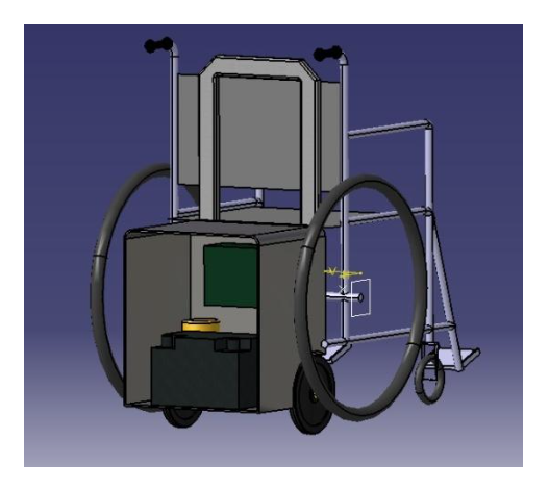
\includegraphics[keepaspectratio=true,scale=0.4]{figuras/estrutura/vista_isometrica_traseira}
\caption{Vista Isométrica Traseira}
\label{fig:vista_isometrica_traseira}
\end{figure}

O objetivo do projeto é desenvolver uma estrutura de fácil conexão e resistente. O produto proposto, ver figura \ref{fig:traseira}, \ref{fig:sistema}, \ref{fig:lateral} e \ref{fig:superior},deve-se acoplar a qualquer cadeira de rodas.

Foi pensado em um dispositivo no formato de uma mala para que seja de fácil conexão, uso e manuseio.

\begin{figure}[!htb]
\centering
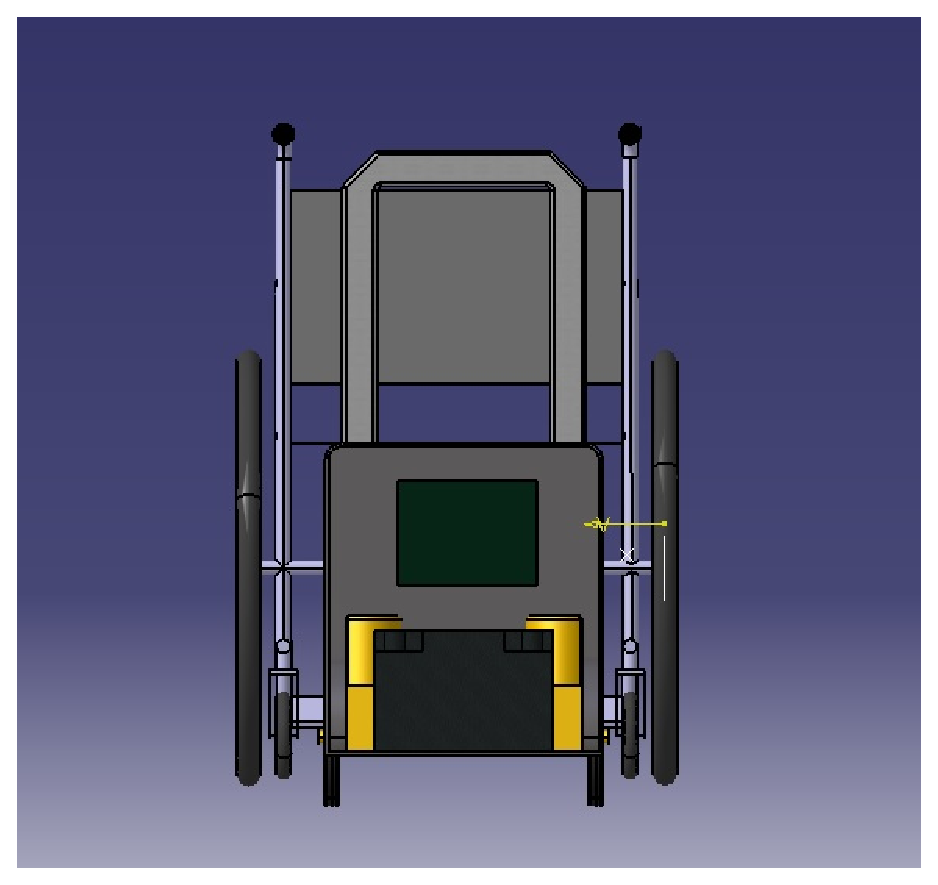
\includegraphics[keepaspectratio=true,scale=0.4]{figuras/estrutura/vista_traseira}
\caption{Vista Traseira}
\label{fig:traseira}
\end{figure}

A forma como a mala será acoplada a cadeira usa como base as hastes da mala e as hastes verticais aonde as manoplas utilizadas para empurrar manualmente a cadeira são fixadas. Tendo em vista que são rígidas e normatizadas pela NBR 9050 as hastes verticais da cadeira tem a distancia e espessura já definidas, o que facilita o desenvolvimento de um produto que possa ser usado em qualquer cadeira de rodas que esteja dentro dos padrões impostos pela norma.

\begin{figure}[!htb]
\centering
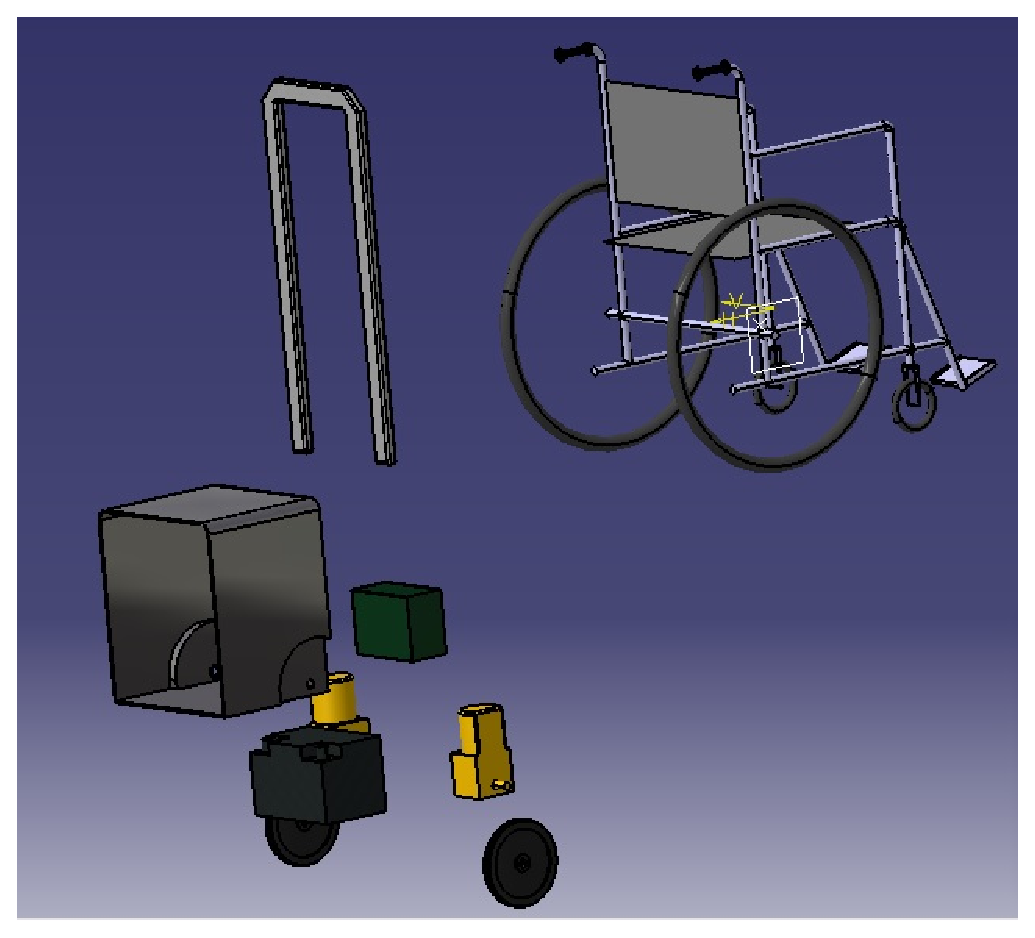
\includegraphics[keepaspectratio=true,scale=0.4]{figuras/estrutura/explode}
\caption{Visão do Sistema}
\label{fig:sistema}
\end{figure}

Cada roda possuirá um motor próprio para que seja possível rotaciona-lás em sentidos opostos, por exemplo, quando for necessário fazer manobras em que a rotação deve ocorre em torno do eixo do próprio cadeirante, movimento muito comum para manobrar uma cadeira de rodas. Assim o cadeirante se sentira confortável e não terá grandes dificuldades quando for manobrar a cadeira, já que a lógica de controle será a mesma usada quando se propulsiona manualmente a cadeira.

\begin{figure}[!htb]
\centering
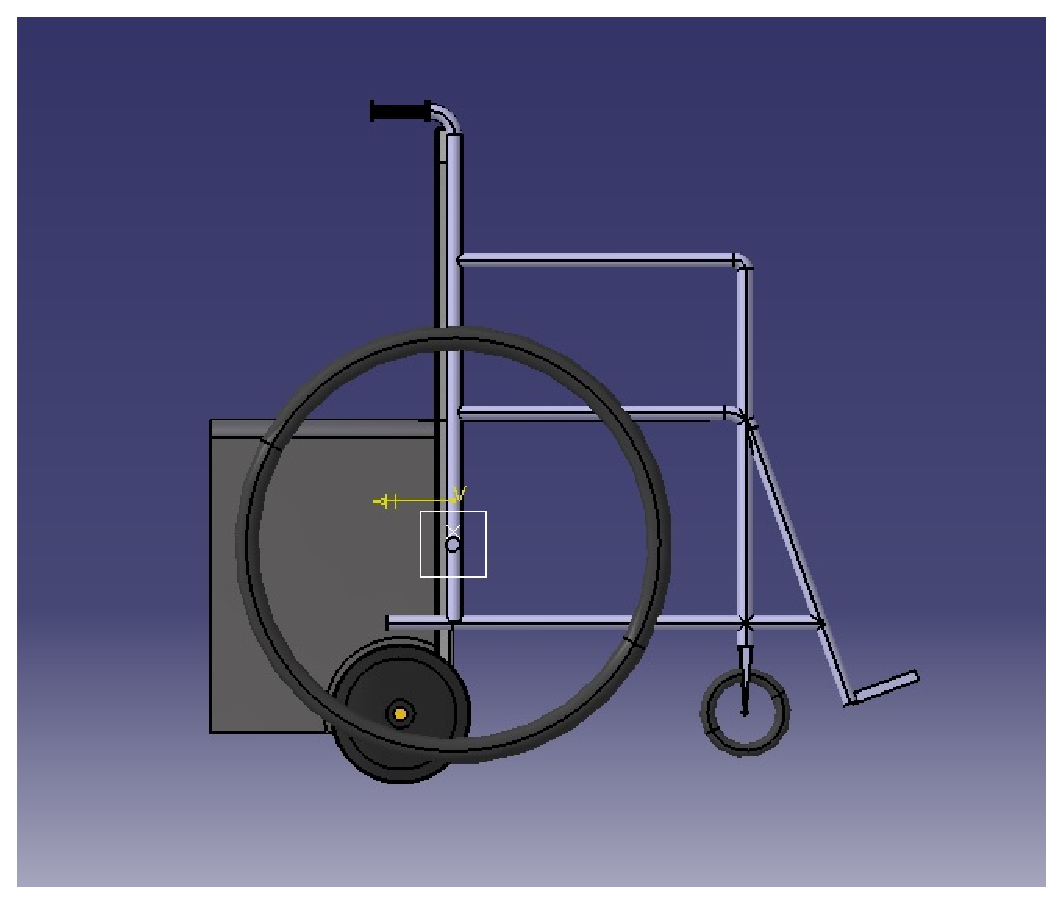
\includegraphics[keepaspectratio=true,scale=0.4]{figuras/estrutura/vista_lateral_cadeira}
\caption{Imagem Lateral}
\label{fig:lateral}
\end{figure}

Como pode se notar nas figuras, o sistema de propulsão devera empurrar a cadeira de rodas, pois assim podemos aproximar o máximo possível o eixo da roda que ira gerar o movimento ao eixo da maior roda da cadeira, o que diminui a quantidade de torque necessário para movimentar o conjunto, fazendo com que o consumo de energia diminua e possibilite o uso de um motor de menor potencia, que diminuirá o custo do produto final.

\begin{figure}[!htb]
\centering
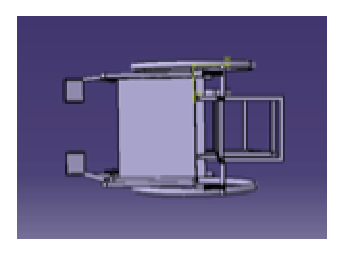
\includegraphics[keepaspectratio=true,scale=0.4]{figuras/estrutura/vista_superior}
\caption{Imagem Superior}
\label{fig:superior}
\end{figure}

\subsection{Protótipo}

A partir do policloreto de vinila, usualmente conhecido como PVC, foi feita uma estrutura de teste para encaixar na parte de trás da cadeira de rodas, com o intuito de buscar a melhor regulação to tamanho da estrutura. O protótipo em questão foi feito para se chegar o mais próximo de um modelo ideal capaz de se acoplar as cadeiras regulamentadas pela NBR 9050.

O protótipo é uma estrutura retangular com uma alça de regulação de largura, seguido de dois “joelhos” em PVC para o acoplamento das rodinhas e da haste, dois encaixes com três saídas para regulação da barra de encaixe superior da cadeira. Há quatro furos na barra de regulação de largura, a qual serve para se adequar ao tipo de cadeira de rodas sendo utilizada, vide figura para mais detalhes \ref{fig:acoplamento}.

\begin{figure}[!htb]
\centering
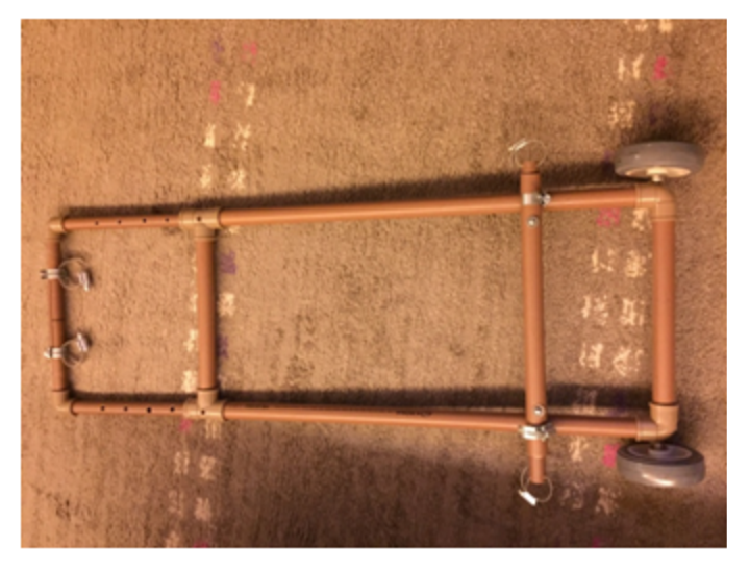
\includegraphics[keepaspectratio=true,scale=0.7]{figuras/resultados/acoplamento}
\caption{Estrutura de acoplamento}
\label{fig:acoplamento}
\end{figure}

No protótipo foram usadas oito braçadeiras circulares de curso infinito, as quais se acoplam na cadeira de rodas dando rigidez a estrutura, dessas oito braçadeiras, duas na parte inferior se acoplam na parte de baixo da cadeira, outras duas se acoplam na parte superior. A figura \ref{fig:acop_bracadeira} ilustra o sistema de acoplamento estrutura/cadeira.

\begin{figure}[!htb]
\centering
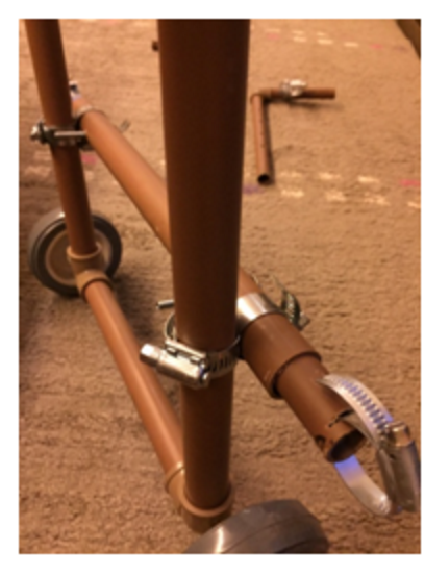
\includegraphics[keepaspectratio=true,scale=0.7]{figuras/resultados/acop_bracadeira}
\caption{Sistema de acoplamento com braçadeira}
\label{fig:acop_bracadeira}
\end{figure}

Na parte da estrutura mostrada na figura \ref{fig:acop_bracadeira} existem dois “joelhos” que ligam as rodinhas com o as barras de PVC, além de uma barra em paralelo com a barra das rodinhas, capaz de variar em altura e largura para se adequar ao tamanho da cadeira utilizada, e  duas braçadeiras nas pontas das barras que irão se acoplar a cadeira de rodas.

\begin{figure}[!htb]
\centering
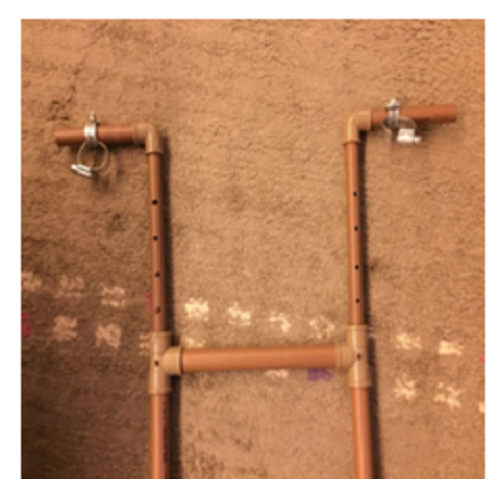
\includegraphics[keepaspectratio=true,scale=0.7]{figuras/resultados/superior_estrutura}
\caption{Parte superior da estrutura}
\label{fig:superior_estrutura}
\end{figure}

A figura \ref{fig:superior_estrutura} representa a parte superior da estrutura, ela contem dois “joelhos” capazes de ligar as duas alças com as duas barras de sustentação da estrutura. Há dois “T” com furo que ligam três barras de cada lado, eles tem a função de regular a altura com o seis furos nas barras de movimentação. Na alça estão duas braçadeiras livres, que se ligam na parte superior da cadeira de rodas, assim como a parte superior já descrita.

Os componentes utilizados para se fazer este modelo são descritos:
\begin{itemize}
  \item Oito braçadeiras circulares de curso infinito;
  \item Quarto “joelhos” de 90$^\circ$;
  \item Dois “T”;
  \item Duas rodas;
  \item Barras de PVC com diâmetros de 20mm e 25mm;
  \item Quatro parafusos;
  \item Oito arruelas;
  \item Quatro porcas.
\end{itemize}

O protótipo apresentado na figura \ref{fig:estr_prototipo} foi capaz de mostrar como funcionará o sistema, e todo encaixe necessário para não ocorrer folga e desconforto ao cadeirante. Esta estrutura se assemelha com as medidas do sistema original, mudando apenas o material da execução e do funcionamento. Obteve-se excelentes resultados testando tal protótipo em dois modelos de cadeira de rodas.

\begin{figure}[!htb]
\centering
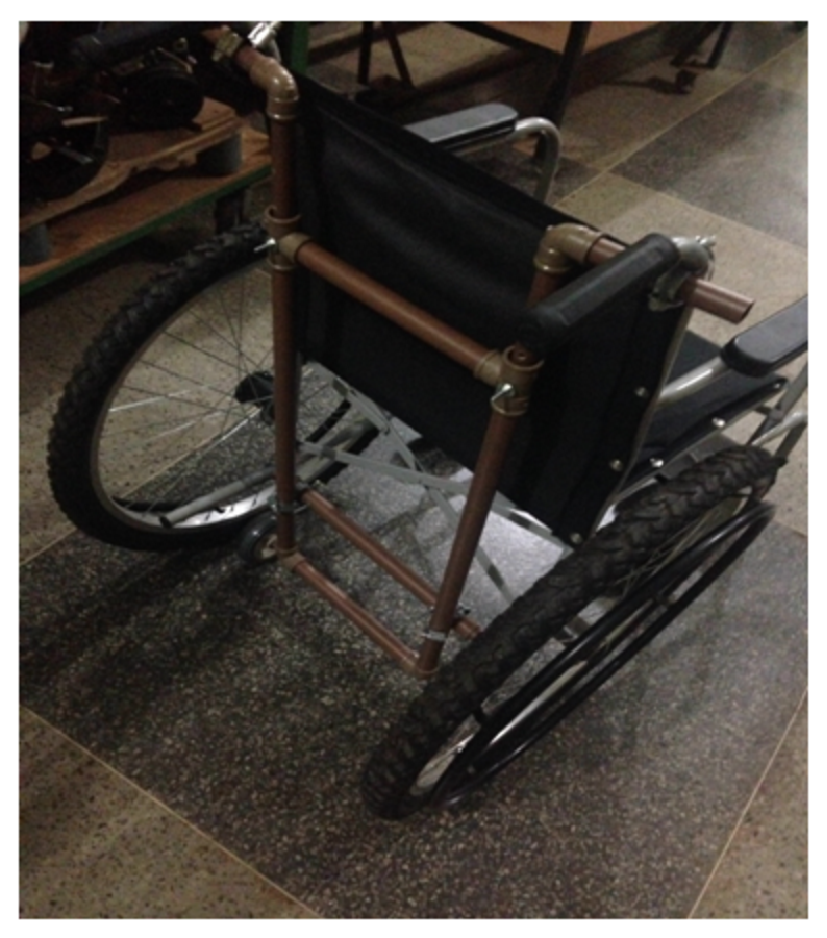
\includegraphics[keepaspectratio=true,scale=0.7]{figuras/resultados/estr_prototipo}
\caption{Estrutura acoplada a cadeira}
\label{fig:estr_prototipo}
\end{figure}

\section{Power-Train}

\subsection{Moto-redutor}

Será utilizado no projeto o motor de corrente contínua. A escolha foi feita pois esse tipo de motor é muito utilizado em projetos que necessitam de velocidades variáveis, eles também apresentam uma região de torque e potência constante e são simples de realizar a aceleração e a desaceleração \cite{manual_bateria_unipower}.

Após uma vasta pesquisa no mercado de motores e redutores, optou-se por comprar dois moto-redutores feitos pela empresa MKS Redutores de São Paulo. O motor com redutor escolhido para o projeto foi o MR com motor GPB que possui as seguintes especificações:

\begin{itemize}
  \item Potência de 305 a 350 W;
  \item 12 ou 24 Vcc;
  \item Rotação de entrada de 2500 rpm;
  \item Reduções de 1:10 até 1:60.
\end{itemize}

Especificações a serem atendidas:

\begin{itemize}
  \item Velocidade máxima de 10 km/h;
  \item 12 Volts corrente contínua;
  \item Peso da bateria 15 kg;
  \item Peso da cadeira (valor aproximado) 15kg;
  \item Peso total estimado: 150 Kg;
  \item Redução de pelo menos 1:10.
\end{itemize}

\subsection{Bateria}

A bateria de chumbo-ácido é muito utilizada hoje em dia em diferentes áreas, como automóveis, sistemas de fornecimento de energia elétrica ininterrupta (no-breaks) e cadeiras de rodas elétricas. Desprezando-se o problema do peso e considerando as observações feitas anteriormente no capítulo \ref{cap:fundamentacao_teorica}, a bateria de chumbo-ácido selada foi a escolhida para o projeto, considerando ainda o seu fácil acesso no mercado e baixo custo.

\subsubsection{Autonomia}

Segundo a literatura, cadeiras de rodas elétricas trabalham com motores de corrente contínua entre 250 W a 300 W de potência. Há diversas maneiras de chegar neste valor, como por distribuição de forças, por balanço de energia, por forças em um plano inclinado, entre outras. Para este projeto fez-se uma estimativa da potência necessária através do balanço de energia [3].

A energia fornecida pelo motor deve ser igual à energia cinética da cadeira. Sendo a massa máxima que a cadeira de rodas aguenta de 150 kg e considerando que cadeiras de rodas elétricas chegam até 10 km/h, tem-se:


\begin{equation}
  Em = \frac{m*V^2*\epsilon}{2}
\end{equation}

Onde $Em$ é a energia fornecida pelo motor, $m$ é a massa de 150 kg e $V$ é a velocidade em metros por segundo. Aqui estimou-se perdas do motor de pelo menos 20\%, sendo assim, $\epsilon$ é igual a 1,20. Assim, a energia necessária para mover a cadeira é de 694 J, a potência é portanto 694 W.

Ao utilizar dois motores de 300 W, a potência total entregue ao sistema seria de 600 W. Rearranjando a equação para encontrar o valor da velocidade, e atribuindo 80\% de eficiência no acoplamento das rodas com o eixo do motor, temos:

\begin{equation}
Em = 0.8*\sqrt{\frac{600*2}{m*\epsilon}}
\end{equation}

Assim, a estimativa da velocidade máxima que a cadeira deve obter será de pelo menos 7.44 km/h, uma velocidade razoável para este tipo de sistema. Sabe-se que a velocidade angular é dada pela divisão da velocidade linear pelo raio:

\begin{equation}
\omega = \frac{V}{r}
\end{equation}

Logo, utilizando a velocidade estimada acima, a velocidade angular obtida é de 20.6 rad/s ou aproximadamente 197 rpm. Considerando as especificações do motor comprado: velocidade angular nominal de 2500 rpm e potência de 305 W, teria de ser feita uma redução de pelo menos 1:10, onde a velocidade angular de saída do redutor seria de 250 rpm. Sendo o torque a divisão da potência pela velocidade angular, o torque gerado é de 29 Nm (Newtons-metro).

Para atender dois motores de 305 W, será conectada uma bateria de carro de chumbo-ácido selado de 12 V (U) e capacidade de 60Ah (I*$\Delta$t), tem-se que a energia $E$ gerada pela bateria é de:

\begin{equation}
E = (I*\Delta t)*U = (60Ah)*12 = 720Wh
\end{equation}

Desta forma, considerando a potência consumida pelos dispositivos eletrônicos de controle desprezível, tem-se que a autonomia da bateria seria de pouco mais de uma hora:

\begin{equation}
\Delta t = \frac{720 Wh}{610 W} = 1.18 h = 1 hora e 10 minutos
\end{equation}

\section{Controle}

\begin{comment}
-------------------------------------------------------------------------------
---- Tópicos para a escrita da parte de controle do capítulo de resultados ----
-------------------------------------------------------------------------------
Panororama do sistema de controle conforme Arquitetura
  - Desde controle de software a periféricos (Usuário a Motor)
  - Panorama de Arquitetura - Antes e depois
    - Citar melhoria quanto ao desempenho
  - Estratégia de comunição entre componentes - Antes e depois
  - Integração Joystick e motor - Falar sobre os estados
\end{comment}

\subsection{Joystick}

O módulo Joystick é a interface de ligação entre o usuário e a cadeira de rodas, este componente é composto por um \textit{joystick} (alavanca que se move sobre uma base e capta movimentos em dois eixos) e um microcontrolador.

Toda a forma de interação entre o usuário e a cadeira de rodas é feita a partir do Joystick, a figura \ref{fig:joy_hand_control} dá uma noção das dimensões e ergonomia deste componente. O controle que fica nas mãos do usuário é conectado à cadeira de rodas por meio de um cabo $RJ45$, apenas o \textit{joystick} foi colocado dentro do controle, o microcontrolador dedicado a este módulo foi colocado junto ao controlador central na traseira da cadeira, para uma maior segurança do mesmo.

\begin{figure}[!htb]
\centering
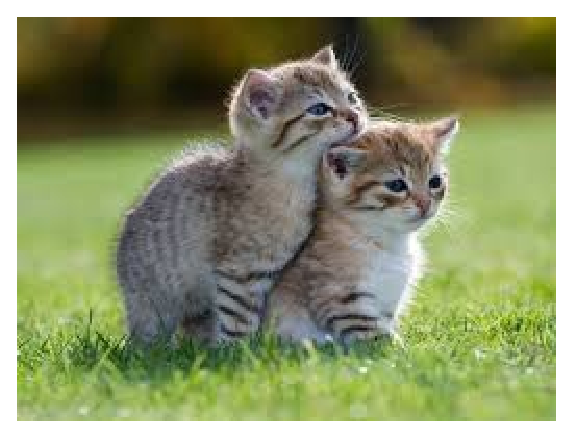
\includegraphics[width = 0.5\textwidth]{figuras/resultados/joy_hand_control}
\caption{Imagem do controle da cadeira de rodas}
\label{fig:joy_hand_control}
\end{figure}

O \textit{joystick} utilizado é composto por dois potenciômetros que indicam as posições em dois eixos independentes. Utilizando os potenciômetros como simples divisores de tensão é possível inferir as posições de seus eixos a partir da medições das tensões do circuito, para realizar esta medição e então rastrear o comando de movimento do usuário, são utilizados dois canais de conversores AD para os potenciômetros, tais conversores são internos ao microcontrolador utilizado e não necessitam de nenhum \textit{hardware} extra.

A rotina de trabalho do microcontrolador do módulo Joystick consiste em adquirir os valores analógicos das posições do \textit{joystick}, convertê-los em valores digitais de um \textit{byte} cada, diferenciando-os utilizando a estratégia de representar um eixo apenas por valores ímpares e o outro apenas por valores pares (ambos entre 0 e 255) e enviá-los via serial alternadamente em um laço infinito, conforme a figura \ref{fig:joy_fluxogram}.

\begin{figure}[!htb]
\centering
\includegraphics[width = 0.9\textwidth]{figuras/resultados/joy_fluxogram}
\caption{Rotina de trabalho do microcontrolador do módulo Joystick}
\label{fig:joy_fluxogram}
\end{figure}

\begin{comment}

Joystick
  - Software e Hardware (periféricos e MSP Joystick)
    - Colocar imagem de código
  - Interface de usuário
    - Fotos do controle

\end{comment}

\subsection{Controlador Central}

  O Raspberry será utilizado como central de comandos para processar as informações vindas do MSP dedicado ao módulo Joystick e enviar o resultado deste processamento para o MSP dedicado aos Motores.

  \textbf{Comunição entre MSP e Raspberry}

  A comunicação, tanto entre o MSP do Josytick e o Raspberry, quanto entre o MSP do Motor e o Raspberry, estão sendo feitas via \textit{threads}.

  A conexão entre os MSP foi formulada através do método \textit{findPort}. Sua implementação pode ser observada na figura \ref{fig:find_port_method}.

  \begin{figure}[!htb]
    \centering
    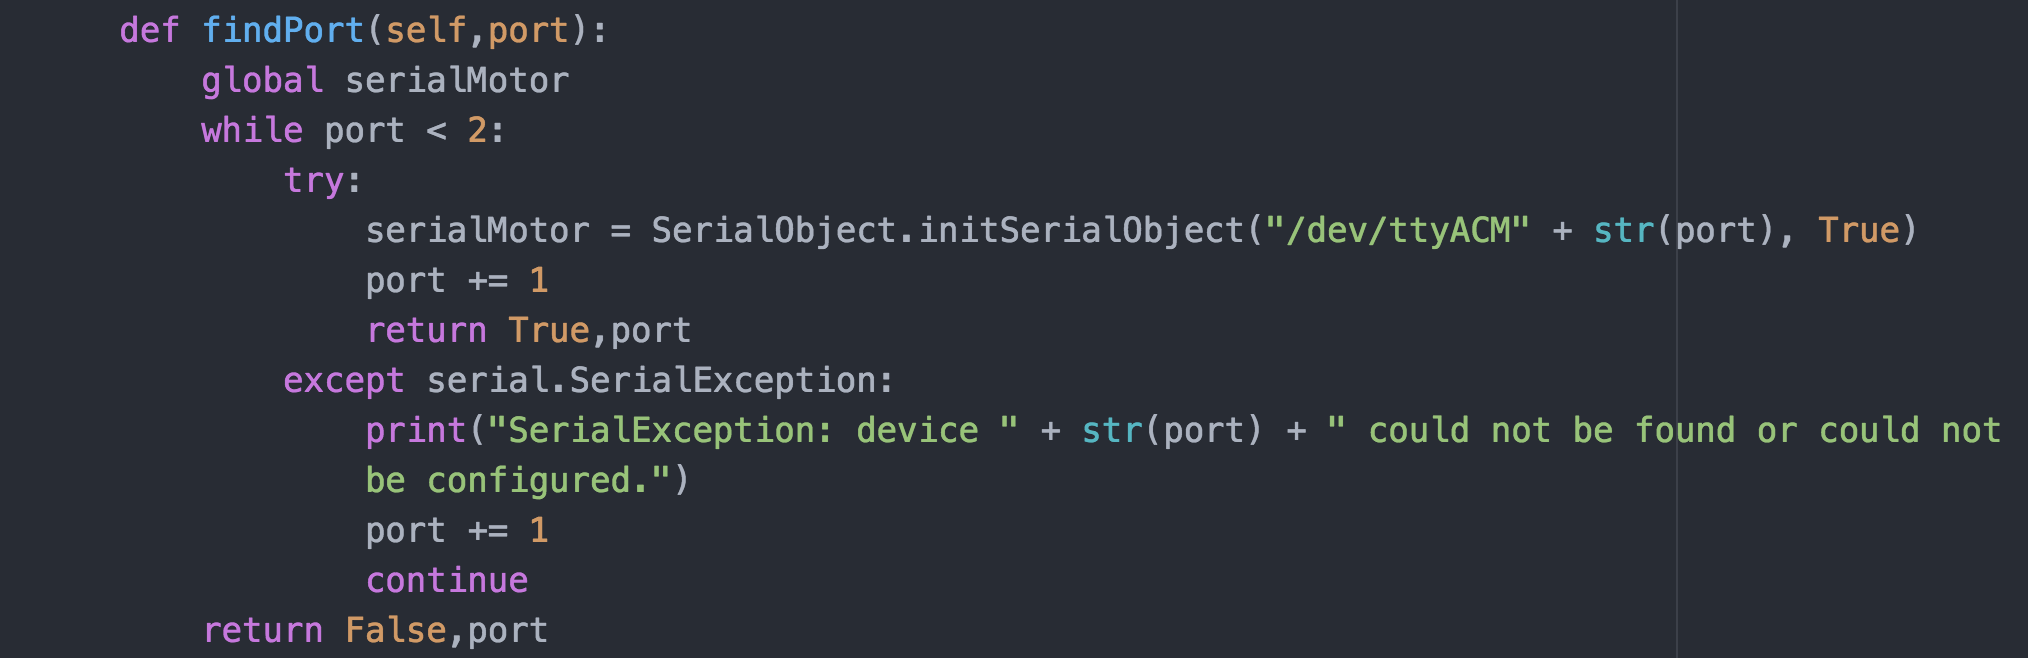
\includegraphics[width=0.9\textwidth]{figuras/resultados/find_port_method}
    \caption{Método para encontrar porta dinamicamente}
    \label{fig:find_port_method}
  \end{figure}

  Este método permite que tanto o MSP do Joystick quanto o MSP do Motor, sejam conectados sem a previa identificação de qual porta utilizar para comunicação. Porém, há existência de prioridade entre as \textit{threads}, ou seja, enquanto a \textit{threads} do Joystick não se conectar com sucesso a \textit{threads} do Motor não irá se conectar.

  Para que este processo ocorra com sucesso, uma checagem de dados é feita para cada tentativa de conexão. Esta checagem consiste em verificar se a porta, a ser conectada, está enviando dados ou recebendo. Para que a conexão do Josytick ocorra com sucesso, a porta deva estar recebendo dados, para que a conexão do Motor ocorra com sucesso, a porta não deve enviar dados. A implementação desta checagem pode ser verificada na figura \ref{fig:try_receive_data}.

  \begin{figure}[!htb]
  \centering
  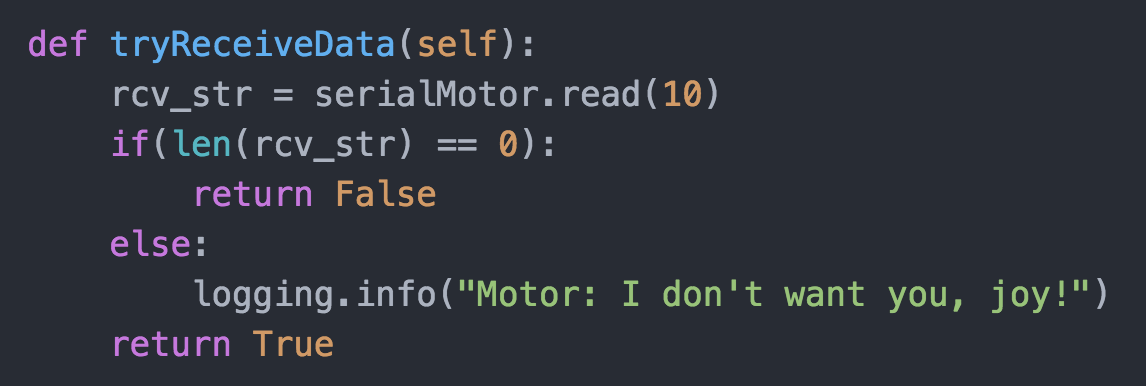
\includegraphics[keepaspectratio=true,scale=0.5]{figuras/resultados/try_receive_data}
  \caption{Método para checar se existe recebimento de dados em porta. Caso do Motor.}
  \label{fig:try_receive_data}
  \end{figure}

  Esta estratégia auxilia na manutenção do produto, pois caso algum MSP fique inutilizavel, é possivel colocar outro MSP, previamente configurado, no lugar do componente inutilizado.

  Após o Raspberry conseguir encontrar uma porta para se conectar com o MSP do Joystick, então a \textit{thread} do MSP do Motor utiliza do mesmo método para se conectar.

  Ao se ter as duas conexões estabelecidas, então o recebimento de dados são adquiridos do Joystick e enviados para os Motores. Para se fazer este envio de informações de forma correta é necessário fazer a sincronização entre as \textit{threads}.

  \textbf{Sincronização de \textit{Threads}}

  Foi percebido que as \textit{threads} precisam estar sincronizadas para se fazer o envio de informações de forma correta. Pois a \textit{thread} do Joystick recebe as informações, e a \textit{thread} do Motor consome estas informações.

  Este problema de sincronização das \textit{threads} é conhecido como um clássico problema de \textit{threads}: Produtor e Consumidor.

  Este problema é caracterizado por 2 processo que compartilharem de um \textit{buffer} comum, no qual o produtor insere a informação no \textit{buffer} e o consumidor retira a informação do \textit{buffer}. Possíveis problemas: Produtor insere produto onde não foi consumido e consumidor remove informação onde já foi removido. Mais detalhes do problema no capítulo \ref{cap:fundamentacao_teorica}.

  Este problema foi solucionado com os seguintes passos:
  \begin{enumerate}
    \item Produtor: Produz os itens necessários em \textit{buffer}, no caso os valores referentes aos potenciometros do Joystick. Neste momento a \textit{thread} do Consumidor é parada e uma variável responsável por esta trava é notificada. Isto pode ser visto na figura \ref{fig:joy_lock};
    \item Consumidor: Consume os itens em \textit{buffer} enviado os mesmos para o MSP dos Motores. Neste momento a \textit{thread} do Produtor é parada e a variável responsável pela trava é consumida. Isto pode ser visto na figura \ref{fig:motor_lock};
  \end{enumerate}

  A variável de trava é utilizada com o propósito de se fazer a produção e o consumo de forma sincronizada. O processo do Consumidor somente será ativo quando o processo do Produtor setar a variável de trava.

  \begin{figure}[!htb]
  \centering
  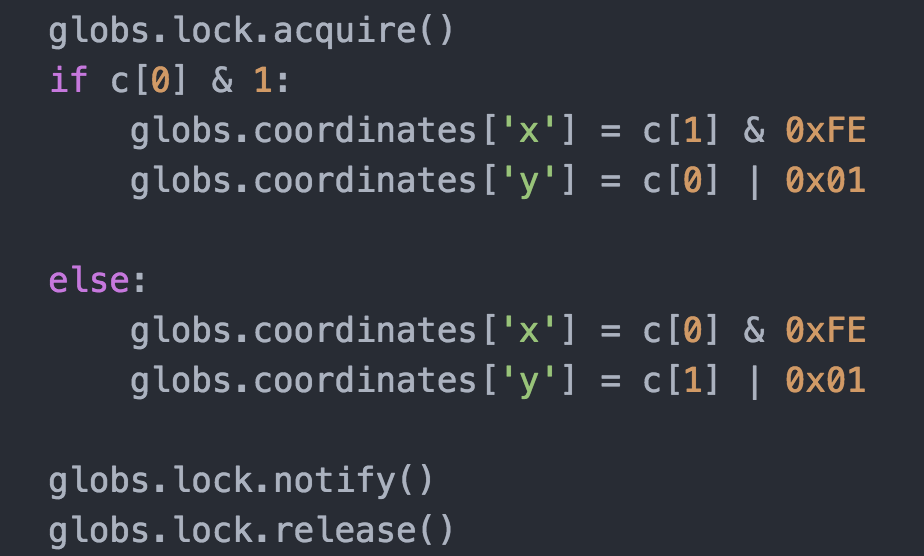
\includegraphics[width=0.9\textwidth]{figuras/resultados/joy_lock}
  \caption{Código utilizado para notificar variável de trava}
  \label{fig:joy_lock}
  \end{figure}

  \begin{figure}[!htb]
  \centering
  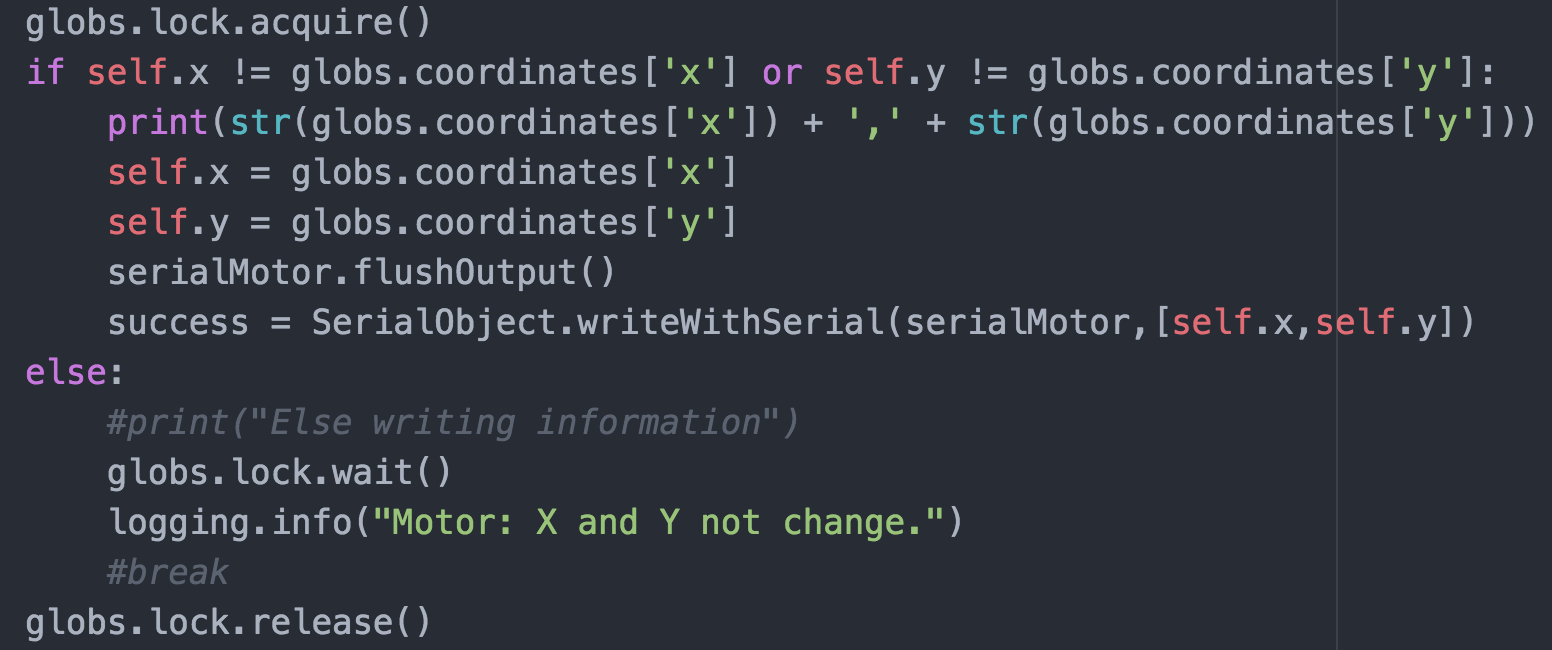
\includegraphics[width=0.9\textwidth]{figuras/resultados/motor_lock}
  \caption{Código utilizado para consumir itens e consequentemente a variável de trava}
  \label{fig:motor_lock}
  \end{figure}


\begin{comment}
Controlador central
  - Explicação de código do Rasp
    - Explicação arquitetura paralela(produtor/consumidor)

Motor
  - Software e Hardware (periféricos e MSP Motor)
    - Colocar imagem de código

Integração Motor e Joystick
  - Mapeamento dos estados em relação ao joystick (255,255->Frente)
  - Mapeamento dos estados em relação aos motores (intensidade, direção)
  - Integração via software ou via hardware
    - Soft
      Vantagens: Uso de propósito geral
      Desvantagem: capacidade de Processamento para cálculo de transformação
    - Hardware:
      Vantagens: Valores de intensidade e direção dos motores são adquiridos de forma instanea
      Desvantagem: Não foi observados desvantagens para a aplicação, porém para outros propósitos é mais dificil de se utilizar os dados, pois os mesmos não tem uma relação direta com o plano cartesiano original.

Ponte-H (copiar e colar do documento pc2)
  - Colocar informações sobre dissipador
  - Estanhamento das placas
  - Dimensionamento da largura das trilhas
  - Circuito de direcionamento das PWMs através das seletoras (demultiplexador)

Alimentação do sistema
  - Esquema de alimentação do sistema
  - Circuito regulador de tensão
\end{comment}
